\chapter{The Scattering of $\alpha$ and $\beta$ Particles by Matter and the Structure of the Atom}

\chapterprecis{Ernest Rutherford}

\makeoddhead{myheadings}{\emph{Rutherford}}{}{\thepage}
\makeevenhead{myheadings}{\thepage}{}{\emph{The Scattering of $\alpha$ and $\beta$ Particles}}

\section*{Remarks}

We have seen how the ``electron'' may be understood as a charged
particle, bearing the fundamental quantity of negative charge, with a
fixed mass that is far smaller than the lightest of atoms. The chemical
or atomic analysis of matter is thus extended to disclose the prospect
of subatomic constituents having both mass and charge.

Accordingly, physics is challenged to interpret the chemical elements as
more or less complex systems of the primordial constituents. How then,
in the atom, are these constituents distributed with respect to one
another? In 1902 Lord Kelvin proposed a model of an electrically neutral
atom containing both positive and negative charge. The positive charge,
and most of the atom's mass, were in this view distributed continuously
throughout the spherical volume of the atom; while the electrons, which
carry negative charge, were embedded in the sphere of positive charge.
Thomson proceeded to investigate this arrangement both mathematically
and experimentally, and it was eventually named after him. The strongest
argument in favor of the Thomson model was that it seemed to explain the
permanence and stability of atoms: Because the electrons were everywhere
surrounded by equal quantities of positive charge the atom would be
electrically neutral in all its parts. A great deal of energy would then
be required to disturb its equilibrium.

Rutherford initially accepted the essential correctness of Thomson's
scheme and set out to verify it experimentally. He and his associates
Geiger and Marsden proposed to bombard individual gold atoms (in fine
gold foils only about 2000 atoms in thickness) with streams of a
radioactive by-product called \emph{alpha particles}. Two kinds of
particles, distinguished as \emph{alpha} and \emph{beta}, are emitted
spontaneously at very high speeds by radium and other radioactive
materials; beta particles were subsequently identified as high-speed
electrons, while the alpha particles proved to be doubly-charged Helium
ions.\footnote{That is, Helium atoms bearing a charge of +2$e$. A
  Helium \emph{ion} is very anomalous from the viewpoint of chemistry,
  for on the electro-chemical interpretation an ion is a
  \emph{chemically active atom}. But Helium is never chemically active!
  The process that produces alpha-particles, then, must involve aspects
  of the atomic structure that chemistry never touches. Furthermore,
  from measurements of their mean free path it
  looked as though $\alpha$-particles were \emph{far smaller} than
  neutral Helium atoms. It takes Rutherford's theory itself to give an
  explanation for this.} Because of their speed and mass alpha-particles
made suitable ``probes'' with which to explore the interior structure of
atoms. By studying the deflections such particles suffered in passing
through gold atoms, Rutherford expected to obtain a more detailed
picture consistent with the Thomson model.

The experiments yielded results that were wholly unexpected. Since the
highest concentrations of mass in the Thomson model are the
\emph{electrons}; and since these are far lighter than alpha particles
and moreover relatively free to move, it was not to be imagined that a
gold atom should be capable of disturbing the path of an alpha particle
by more than a fraction of a degree. But in fact, prodigious deviations
were observed, some greater than $90^\circ$. And these deflections occurred,
moreover, with a frequency some 104596 times greater than the
probability as calculated according to Thomson's arrangement.
Rutherford, later in life, expressed his astonishment as follows:

\begin{quote}
It was quite the most incredible event that ever happened to me in my
whole life. It was as incredible as if you fired a 15-inch shell at a
piece of tissue paper and it came back and hit you. On consideration I
realized that the scattering backwards must be the result of a single
collision, and when I made the calculation I saw that it was impossible
to get anything of that order of magnitude unless you took a system in
which the greater part of the mass of the atom was concentrated in a
single nucleus. It was then that I had the idea of an atom with a minute
massive center carrying a charge.
\end{quote}

\subsection*{A Note on Probability\footnote{Note by Michael Comenetz}}

A reader of Ernest Rutherford's famous paper \emph{The Scattering of $\alpha$
and $\beta$ Particles by Matter and the Structure of the Atom}, which reports
the discovery of the atomic nucleus, may be perplexed by a couple of
expressions at the beginning of §3. An explanation follows.

\begin{figure}[h]
  \begin{center}
    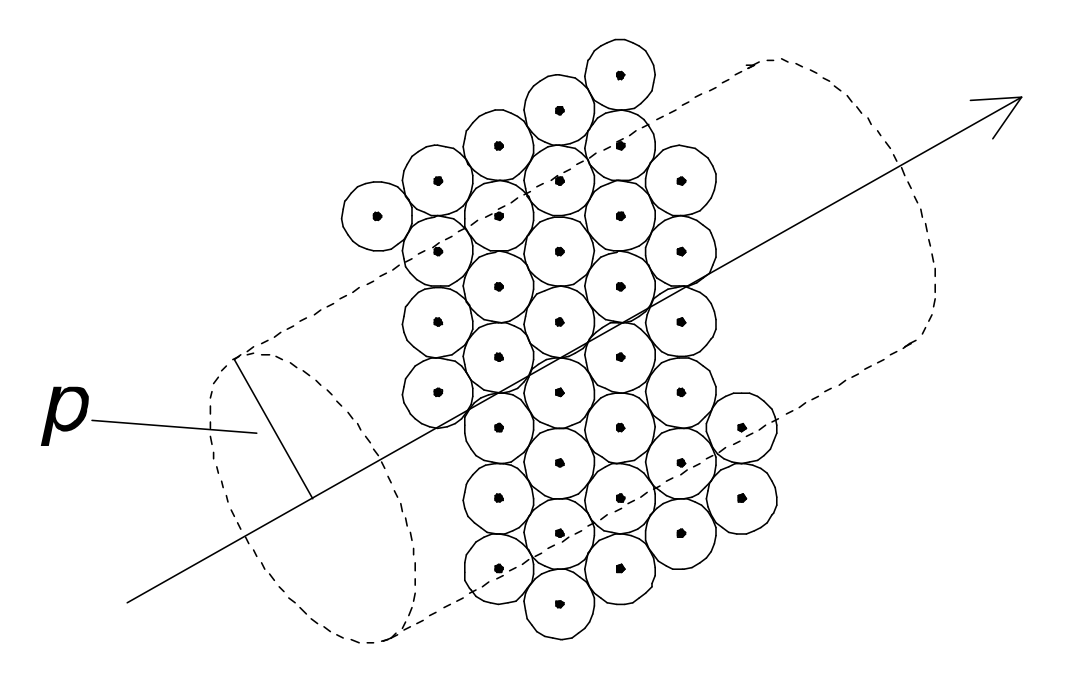
\includegraphics[width=2.1875in,height=1.57292in]{images/04_rutherford/collisions.png}
  \end{center}
    \caption*{\emph{An alpha particle and its presumptive path
      through a section of gold foil. You should imagine the atomic centers 
      as being more randomly arrayed.}}
\end{figure}

We are playing a game of shooting tiny particles at a thin screen of
large spherical atoms, in the direction normal (perpendicular) to its
surface. With very few exceptions, the particles pass straight through
the screen; for our present purpose we assume that all do. Having chosen
a distance $d$, we say that a particle \emph{hits} an atom if it
comes within that distance of the center of the atom. For a given shot,
our \emph{score} is the number of atoms hit by the particle. Each shot
is taken in the same way, and the shots are independent of one
another---the score for one shot has no influence on the score for
another.

When we take a number of shots, our \emph{average score} means the
result of dividing the total of our scores by the number of shots. For
example, if we score successively 2, 0, 5, 2, 0, 2, 3, our total score
is 14 and the number of shots is 7, so our average score~is 2. If we
score successively 1, 0, 0, 0, 1, 0, 1, 0, our total score is 3 and the
number of shots is 8, so our average score~is 0.375.

Since the shots are alike and independent, it is reasonable to suppose
that as we take more and more of them, our average score will approach
some definite value as a limit. The limiting value can be called our
\emph{expected score}, or \emph{expectation}, because when we play the
game, we expect our scores to cluster around that value, and our average
score to tend towards it. The expectation, which we call $e$, will
be well approximated by the average score we get when we take a large
number of shots.

In order to estimate the expectation, let us call the thickness of the
screen $t$, and the density of atoms within it $N$. The latter
quantity means the average number of atoms per unit volume; that is the
same as the average number of centers of atoms per unit volume.

The question, ``On average, how many atoms does a particle hit?'' is
equivalent to the question, ``On average, how many atom-centers lie
within distance $d$ of the path of the particle?'' and therefore
also to the question, ``On average, how many atom-centers lie within the
right circular cylinder of radius $d$ whose axis is the path of the
particle through the screen, and whose height is the thickness $t$
of the screen?''

The volume of such a cylinder---that is, the number of unit volumes it
contains---is the area of its base, which is
$\pi d^2$, times its height $t$, or
$\pi d^{2}t$. It follows that the average
number of atom-centers in such a cylinder is
$n \times \pi d^{2}t = \pi d^{2}nt$. This is then our
expectation: $E = \pi d^{2}nt$

We now apply this result to two special cases.

\textbf{Case 1.}~ Let $d$ be the radius $R$ of an atom. In
this case, \emph{hitting} an atom has the ordinary sense of coming into
contact with it. The expectation $e$ is
$\pi R^{2}nt$. This is what
Rutherford means by saying that ``the number of collisions of the
particle with the atom of radius $R$ is
$\pi R^{2}nt$.'' The value of
$e$ is of the order of the number of atoms spanning the thickness
$t$---a few thousand, for a gold-foil screen.

\textbf{Case 2.}~ Let $d$ be a distance $p$ much smaller than
$R$, a thousand or ten thousand times smaller. In this case it is
very difficult to \emph{hit} an atom---so difficult, that we may assume
that no particle hits more than one. Then for each shot our score is 0
or 1, and the expectation $E = \pi p^{2}nt$ has a value between 0
and 1.

Since in this case there are only two possibilities for each shot,
either it hits or it doesn't, we can speak of the \emph{probability}
$p$ that a given shot will hit an atom, understanding by this the
proportion of hits, or average score, obtained when a great many shots
are taken (more precisely, its limiting value as the number of shots
increases)---that is, the expectation: $p$ = $e$. If we
assert, for example, that $p$ = 0.20, or 20\%, we expect that out
of, say, 1000 shots, there will be about 200 hits---that the average
score for those 1000 shots will be about 200/1000 = 0.20, that about
20\% of them will be hits. Hence Rutherford writes, ``The probability
\ldots{} of entering an atom within distance $p$ of its centre is
given by \ldots{} $\pi p^{2}nt.$''\footnote{See page
  67.}

\subsection*{Final Thoughts}

1. The assumption in the first paragraph of the explanation is
justified as follows. A particle deviates appreciably from a straight
path only if it hits an atom for very small $d$, as in Case 2. Even
if so deflected, it is very unlikely to hit another atom, because
$d$ is much less than $R$ and $t$ is very small. Thus
only the possibility of a first encounter along a straight path need be
admitted.

2. One may wonder why probability enters the picture only with Case 2.
Shouldn't the general case somehow involve probability? It does. Let
$N$ be the greatest number of atoms the particle can possibly hit.
Let $p_0$ be the probability that it hits no atoms,
$p_1$ the probability that it hits exactly one,
$p_2$ the probability that it hits exactly two,
\ldots{}, \emph{P\textsubscript{N}} the probability that it hits exactly
$N$. Then $p_0$ + $p_1$ +
$p_2$ + $\cdot \cdot \cdot$ + $P_N$ = 1 and
$p_0$ $\cdot$ 0 + $p_1$$\cdot$1 +
$p_2$$\cdot$2 + $\cdot \cdot \cdot$
+~\emph{P\textsubscript{N}}$\cdot$$N$ = $e$. In Case 2, the only
non-zero probabilities are $p_0$ and
$p_1$, hence $p_1$ = $e$.

3. The intuitive understanding of expectation as the limit of the
average score rests on the assumption stated in the third paragraph,
that the limit exists. In the mathematical theory of probability a
different approach is taken, and the limit assertion becomes a theorem,
or rather a class of theorems (\emph{laws of large numbers}).


\section*{The Scattering of $\alpha$ and $\beta$ Particles by Matter\\
  and the Structure of the Atom\footnote{{[}\emph{Philosophical Magazine}
  \textbf{211} (1911), 669--688.{]}}\\
  {\large Ernest Rutherford}}



\S1. It is well known that the $\alpha$ and $\beta$ particles suffer
deflexions from their rectilinear paths by encounters with atoms of
matter. This scattering is far more marked for the $\beta$~than for the
$\alpha$~particle on account of the much smaller momentum and energy of
the former particle. There seems to be no doubt that such swiftly moving
particles pass through the atoms in their path, and that the deflexions
observed are due to the strong electric field traversed within the
atomic system. It has generally been supposed that the scattering of a
pencil of $\alpha$~or $\beta$~rays in passing through a thin plate of
matter is the result of a multitude of small scatterings by the atoms of
matter traversed. The observations, however, of Geiger and Marsden on
the scattering of $\alpha$~rays indicate that some of the $\alpha$
particles must suffer a deflexion of more than a right angle in a single
encounter. They found, for example, that a small fraction of the
incident $\alpha$~particles, about 1 in 20,000, were turned through an
average angle of 90$^\circ$ in passing through a layer of gold-foil about
.00004 cm. thick, which was equivalent in stopping-power of the
$\alpha$~particle to 1.6 millimetres of air. Geiger showed later that
the most probable angle of deflexion for a pencil of $\alpha$ particles
traversing a gold-foil of this thickness was about 0$^\circ$.87.\footnote{{[}That
  is, particles passing through the foil were deflected within, say, .1$^\circ$
  of 0.87$^\circ$ more often than within .1$^\circ$ of any other angle.{]}} A simple
calculation based on the theory of probabilities shows that the chance
of an $\alpha$~particle being deflected through 90$^\circ$ {[}as the cumulative
result of multiple encounters{]} is vanishingly small.\footnote{{[}If
  $\theta_0$ is the most probable angle of deflection resulting from many
  atomic encounters, a general theorem holds that the probability of
  obtaining a deflection angle of any other value $\theta$~or greater is
  $e^{-(\theta/\theta_0)^2}$. Since Geiger has shown that $\theta_0 = .87^{\circ}$, the probability of
  obtaining $\theta = 90^\circ$ will be or about $10^-{4600}$.{]}} In addition, it
will be seen later that the distribution of the $\alpha$ particles for
various angles of large deflexion does not follow the probability law to
be expected if such large deflexions are made up of a large number of
small deviations. It seems reasonable to suppose that the deflexion
through a large angle is due to a single atomic encounter, for the
chance of a second encounter of a kind to produce a large deflexion must
in most cases be exceedingly small. A simple calculation shows that the
atom must be the seat of an intense electric field in order to produce
such a large deflexion at a single encounter.

Recently Sir J.\ J.\ Thomson has put forward a theory to explain the
scattering of electrified particles in passing through small thicknesses
of matter. The atom is supposed to consist of a number $N$ of
negatively charged corpuscles, accompanied by an equal quantity of
positive electricity uniformly distributed throughout a sphere. The
deflexion of a negatively electrified particle in passing through the
atom is ascribed to two causes---(1) the repulsion of the corpuscles
distributed through the atom, and (2) the attraction of the positive
electricity in the atom. The deflexion of the particle in passing
through the atom is supposed to be small, while the average deflexion
after a large number $m$ of encounters was taken as
$\sqrt{m} \cdot \theta$, where $\theta$ is the average deflexion due to a
single atom. It was shown that the number $N$ of the electrons
within the atom could be deduced from observations of the scattering of
electrified particles. The accuracy of this theory of compound
scattering was examined experimentally by Crowther in a later paper. His
results apparently confirmed the main conclusions of the theory, and he
deduced, on the assumption that the positive electricity was continuous,
that the number of electrons in an atom was about three times its atomic
weight.

The theory of Sir J.~J. Thomson is based on the assumption that the
scattering due to a single atomic encounter is small, and the particular
structure assumed for the atom does not admit of a very large deflexion
of an $\alpha$ particle in traversing a single atom, unless it be
supposed that the diameter of the sphere of positive electricity is
minute compared with the diameter of the sphere of influence of the
atom.

Since the $\alpha$ and $\beta$ particles traverse the atom, it should
be possible from a close study of the nature of the deflexion to form
some idea of the constitution of the atom to produce the effects
observed. In fact, the scattering of high-speed charged particles by the
atoms of matter is one of the most promising methods of attack of this
problem. The development of the scintillation method\footnote{{[}The
  \emph{scintillation method}: an alpha-particle is made to strike a
  zinc sulphide screen, which then gives off a tiny flash of light. The
  flash is observed with a microscope, and the number of particles
  incident on any given area in a given time interval are thus
  counted.{]}} of counting single $\alpha$ particles affords unusual
advantages of investigation, and the researches of H. Geiger by this
method have already added much to our knowledge of the scattering of
$\alpha$ rays by matter.

\smallskip

\S2. We shall first examine theoretically single encounters\footnote{The
  deviation of a particle through a considerable angle from an encounter
  with a single atom will in this paper be called ``single'' scattering.
  The deviation of a particle resulting from a multitude of small
  deviations will be termed ``compound'' scattering.} with an atom of
simple structure, which is able to produce large deflexions of an
$\alpha$~particle, and then compare the deductions from the theory with
the experimental data available.

Consider an atom which contains a charge $\pm Ne$ at its centre
surrounded by a sphere of electrification containing a charge $\mp Ne$
supposed uniformly distributed throughout a sphere of radius $R$.
$e$ is the fundamental unit of charge, which in this paper is taken
as $4.65 \times  10^{-10}$ \textsc{e.s.} unit. We shall suppose that for distances
{[}greater{]}\footnote{{[}We here correct a typographical error in the
  original.{]}} than $10^{-12}$ cm. the central charge and also the charge on
the~$\alpha$ particle may be supposed to be concentrated at a point. It
will be shown that the main deductions from the theory are independent
of whether the central charge is supposed to be positive or negative.
For convenience, the sign will be assumed to be positive. The question
of the stability of the atom proposed need not be considered at this
stage, for this will obviously depend upon the minute structure of the
atom, and on the motion of the constituent charged parts.

In order to form some idea of the forces required to deflect an
$\alpha$~particle through a large angle, consider an atom containing a
positive charge $Ne$ at its centre, and surrounded by a
distribution of negative electricity $Ne$ uniformly distributed
within a sphere of radius $R$. The electric {[}field{]} \emph{X}
and the potential $V$ at a distance $R$ from the centre of an
atom, for a point inside the atom, are given by\footnote{{[}Rutherford's
  actual expression is ``electric force $X$.'' But what he is
  actually calculating is the \emph{intensity} of the force---the force
  per unit charge---and thus $X$ really represents \emph{electric
  field strength}. See App. II B below.
  
  The atom is assumed to contain $N$ negative electrons evenly
  distributed throughout its volume and $N$ positive charges
  concentrated in the nucleus. Thus the electric field within the atom
  at a distance $r$ from the nucleus has two sources: (a) the
  nucleus, and (b) those electrons that are contained \emph{within}
  radius $R$. (Electrons lying \emph{beyond} radius $R$ make
  no contribution to the field at $R$, for the electric field
  within any closed, charged surface is \emph{zero}; compare the
  analogous case for gravitation, Newton's \emph{Principia}, Book I,
  Prop.\ 70.)
  
  Now (a) the electric field intensity due to the positive nucleus is
  $Ne/r^2$. And the negative charge contained within radius
  $r$ is to $Ne$ as the volume of the sphere of radius
  $r$ is to the whole atom; hence that charge is
  $-Ne(r^3/R^3)$. It acts as though it were
  concentrated at the center (see \emph{Principia}, Book I, Prop.\ 71);
  therefore (b) its contribution to the electric field intensity is
  $-Ne(r^3/R^3)/r^2$ or $-Ne(r/R^3)$. The total electric field intensity
  $X$ is the sum of (a) and (b), as in Rutherford's expression.{]}}
%
\begin{equation*}
X = Ne\left(\frac{1}{r^2} - \frac{r}{R^3}\right)
\end{equation*}
%
{[}and{]}\footnote{[To determine the electric potential we
  \emph{integrate} the field strength $X$ \emph{over distance} (see
  Appendix II B, 269-71 below for a discussion of this), from $s = r$ 
  to $s = R$ (it is not necessary to consider radii
  greater than $R$ because, the atom as a whole being electrically
  neutral, there is no field beyond $R$). Thus Rutherford's
  expression for $V$ is the result of having evaluated the integral
  $\int_{r}^{R} \! Ne(1/s^2 - s/R^3)\,ds$ .]}

\begin{equation*}
V = Ne\left(\frac{1}{r} - \frac{3}{2R} + \frac{r^2}{2R^3}\right).
\end{equation*}

Suppose an $\alpha$~particle of mass $m$ and velocity \emph{u} and
charge $e$ shot directly towards the centre of the atom. It will be
brought to rest at a distance $b$ from the centre given
by\footnote{{[}The work required to bring a positive charge $e$
  from infinity to a distance $r$ from the center of the atom is
  given by the product $VE$ of the charge and the electric
  potential at the distance $r$---again see Appendix II B. If this
  work is done at the expense of the incident particle's kinetic energy,
  the particle will be brought to rest (at distance $b$ from the
  center) when the initial kinetic energy of the particle equals
  \emph{VE}, that is, when
  \begin{equation*}
  \frac{1}{2}mu^2 = VE = NeE\left(\frac{1}{b}-\frac{3}{2R}+\frac{b^2}{2R^3}\right).]
  \end{equation*}}

\begin{equation*}
\frac{1}{2}mu^2 = NeE\left(\frac{1}{b} - \frac{3}{2R} + \frac{b^2}{2R^3}\right).
\end{equation*}

It will be seen that $b$ is an important quantity in later
calculations. Assuming that the central charge is 100$e$, it can be
calculated that the value of $b$ for an $\alpha$~particle of
velocity $2.09 \times 10^9$ cm. per second is about $3.4 \times 10^{-12}$ cm. In this
calculation $b$ is supposed to be very small compared with
$R$. Since $R$ is supposed to be of the order of the radius of
the atom, viz.\ $10^{-8}$ cm., it is obvious that the $\alpha$~particle before
being turned back penetrates so close to the central charge, that the
field due to the uniform distribution of negative electricity may be
neglected. In general, a simple calculation shows that for all
deflexions greater than a degree, we may without sensible error suppose
the deflexion due to the field of the central charge alone.\footnote{{[}Since
  Rutherford has concluded that $b$ ($\approx 10^{-12}$ cm.)
  is very small in comparison with $R$ ($\approx 10^{-8}$
  cm.), he ignores the last two terms in parentheses in the equation
  above; thus
  \begin{equation*}
  b = 2NeE/mu^2
  \end{equation*}
  This is equivalent to assuming that the electric potential $V$ at
  $b$ was equal to $Ne/b$ and thus that it was due to the
  field of the central charge alone. Rutherford will make use of this
  expression for $b$ below.]} Possible single deviations 
  due to the negative electricity, if distributed in the form
of corpuscles, are not taken into account at this stage of the theory.
It will be shown later that its effect is in general small compared with
that due to the central field.

%
\begin{figure}[h]
  \begin{center}
    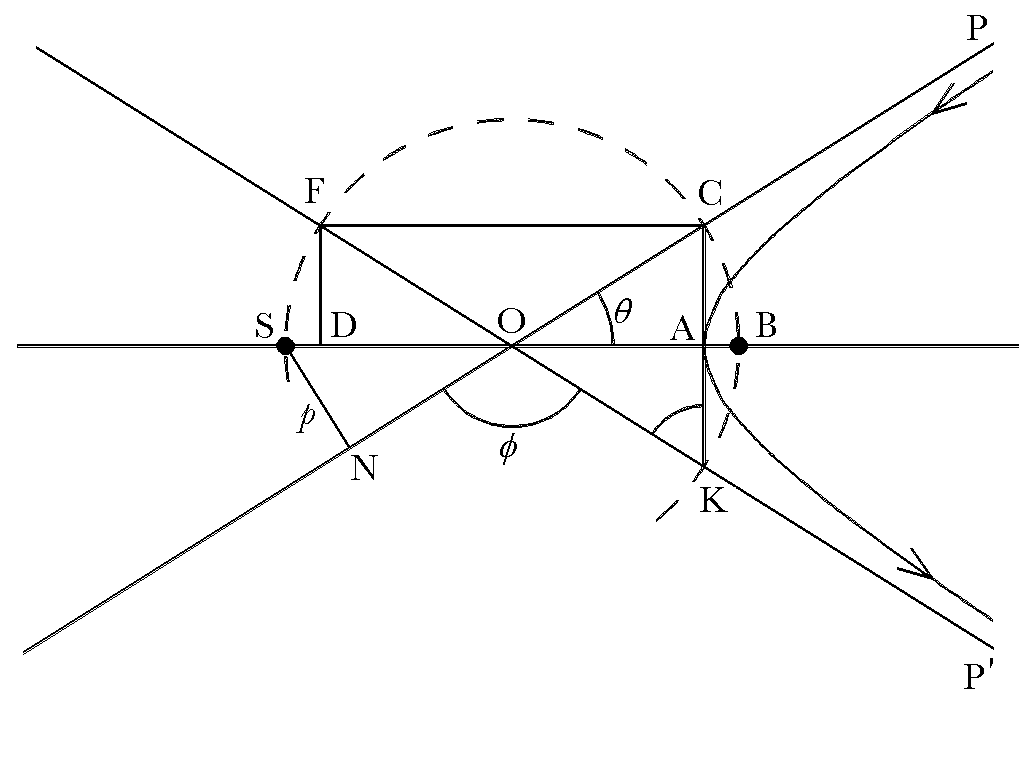
\includegraphics[width=4.65625in,height=3.5in]{images/04_rutherford/image005.png}
  \end{center}
    \caption*{Figure 1}
\end{figure}
%

Consider the passage of a positive electrified particle close to the
centre of an atom. Supposing that the velocity of the particle is not
appreciably changed by its passage through the atom, the path of the
particle under the influence of a repulsive force varying inversely as
the square of the distance will be an hyperbola\footnote{{[}Newton,
  \emph{Principia}, Cor. I, Prop.\ 13. Note also that the force being
  repulsive (``centrifugal''), Newton's Scholium after Prop.\ 10 applies
  to determine the conic as a hyperbola.{]}} with the centre of the atom
S as the external focus. Suppose the particle to enter the atom in the
direction PO {[}Fig.1{]},\footnote{{[}In Figure 1 we have added
  auxiliary elements in order to apply propositions from Apollonius'
  \emph{Conics}. Rutherford himself argues trigonometrically.\\
  We show that B, C, and S lie on the circumference of a circle as follows: 
  By Apollonius III.45 and II.1,
  rect. DB,BA and sq. AC are each equal to 1/4 ``the figure'' and
  therefore are equal to each other. But DB = OB + OA and BA = OB - OA;
  hence\\
	\begin{equation*}
   (\text{AC})^2 = \text{DB} \cdot \text{BA} = (\text{OB} + \text{OA})(\text{OB} - \text{OA}) = (\text{OB})^2 - (\text{OA})^2 .
	\end{equation*}
  But in rt. triangle OAC,
  \begin{equation*}
  (\text{AC})^2 = (\text{OC})^2 - (\text{OA})^2 .
  \end{equation*}
  Then (OC)$^2$ = (OB)$^2$ and OC = OB. Similarly OC = OS also. Thus OC = OB =
  OS , so that a circle about O will pass through the points K, B, C, F,
  S as shown in the drawing. Q.E.D.{]}} and that the direction of motion
on escaping the atom is OP'. OP and OP' make equal angles with the line
SA, where A is the apse {[}vertex{]} of the hyperbola. $p$ = SN =
perpendicular distance from centre on direction of initial motion of
particle.

Let angle POA = $\theta$.

Let $u$ = velocity of particle on entering the atom,\footnote{{[}Rutherford
  actually writes $V$ at this point, not $u$, to represent the
  initial velocity of the alpha particle! But since he used $u$ to
  denote that velocity on p. 67 above, and $V$ to represent the
  \emph{electric potential}, we will retain his original meanings for
  $u$ and $V$ throughout.{]}} $v$ its velocity at A, then
from consideration of angular momentum

\begin{equation*}
pu = \text{SA} \cdot v .\footnote{{[}Newton, \emph{Principia}, Cor.
  I, Prop.\ I states that if a body is acted on by a central force, its
  velocity at different points along its path varies inversely as the
  perpendiculars dropped from the center of force to the tangents to the
  body's path at those points. Here SA is the perpendicular dropped from
  S to the tangent at A; SN ($= p$) is the perpendicular dropped
  from S to the asymptote, which is nearly the same as the tangent at
  some extremely distant point. Thus
  \begin{tabular}{c c c}
  $u : v :: \text{SA} : \text{SN}$ &  or & $u: v :: \text{SA} : p$\\
  \end{tabular}
  Rutherford's equation follows by equating the products of means and
  extremes. These products are said to express the \emph{angular
  momentum} of the body at the points in question.{]}}
\end{equation*}

From conservation of energy\footnote{{[}The alpha-particle, starting its
  trajectory far from the atomic center, is considered to have initial
  potential energy \emph{zero}. When it reaches vertex A it will have
  potential energy \emph{NeE}/SA, equal to its loss of kinetic energy,
  $(1/2)mu^2 = (1/2)mv^2${]}}
\begin{equation*}
\frac{1}{2}mu^2 = \frac{1}{2}mv^2 + \frac{NeE}{SA}.
\end{equation*}
{[}Now, since $NeE = (1/2)mu^2b$,{]}\footnote{{[}In
  note 13 above we found
  \begin{equation*}
  b = 2NeE/mu^2; \quad\text{that is,}\quad NeE = bmu^2.
  \end{equation*}
  Hence, substituting into the previous equation,
  \begin{equation*}
  (1/2)mu^2 - (1/2)mv^2 = bmu^2/2\cdot \text{SA}, \quad\text{or}\quad v^2 = u^2(1-b/\text{SA}).
  \end{equation*}{]}}
  \begin{equation*}
  v^2 = u^2 \left( 1-\frac{b}{\text{SA}} \right) .
  \end{equation*}\\
\centerline{* * *}
%
{[}Therefore also{]}
\begin{equation*}
p^2 = \text{SA} \cdot (\text{SA} - b) .\footnote{[In $pu = \text{SA} \cdot v$ from above, square both sides to obtain
  \begin{equation*}
  p^2u^2 = (\text{SA})^2v^2.
  \end{equation*}
  But
  \begin{equation*}
  v^2 = u^2(1-b/\text{SA}),
  \end{equation*}
  as was just derived. Therefore,
  \begin{equation*}
  p^2u^2 = (\text{SA})^2 \cdot u^2(1-b/\text{SA})
  \end{equation*}
  or
  \begin{equation*}
  p^2 = \text{SA} \cdot (\text{SA} - b).
  \end{equation*}]}
\end{equation*}\\
\centerline{* * *}
%
The angle of deviation $\phi$~of the particle is $\pi - 2\theta$ and
\begin{equation*}\tag{1}
\cot{\phi/2} = 2p/b.\footnote{[In Figure 1, $\triangle$ OAC $\cong$ $\triangle$ ONS;
  therefore SN = AC. But AC is a mean proportional between segments
  SA,AB since it is perpendicular to the circle diameter SB. Hence SN,
  that is $p$, is likewise a mean proportional between the same two
  segments, or
  \begin{equation*}
  p^2 = \text{SA} \cdot \text{AB}.
  \end{equation*}
  But we just saw, above,
  \begin{equation*}
  p^2 = \text{SA} \cdot (\text{SA} - b)
  \end{equation*}
  so it must be the case that
  \begin{equation*}
  \text{AB} = \text{SA} - b,
  \end{equation*}
  that is,
  \begin{equation*}
  b = \text{SA} - \text{AB} = \text{SA} - \text{SD} = \text{DA}.
  \end{equation*}
  Now since $p = \text{AC}$ and $b = \text{DA}$,
  \begin{equation*}
  2p/b = 2 \cdot \text{AC/DA} = \text{KC/CF} = \tan \angle \text{CFK} = \cot \angle \text{CKF} = \cot \phi/2.{]}
  \end{equation*}}\footnote{A simple consideration shows that the deflexion is
  unaltered if the forces are attractive instead of repulsive.
  {[}Compare Newton, \emph{Principia}, Book I, Prop.\ 12, ``The Same
  Otherwise'': ``And the same way it may be demonstrated, that the body
  having its centripetal changed into a centrifugal force, will move in
  the opposite branch of the hyperbola.''{]}}
  \end{equation*}

This gives the angle of deviation of the particle in terms of $b$,
and the perpendicular distance of the direction of projection from the
centre of the atom.

For illustration, the angles of deviation $\phi$~for different values
of $p/b$ are shown in the following table:---
\begin{center}
\begin{tabular}{c c c c c c c c}
$p/b$ & 10 & 5  & 2 & 1 & .5 & .25 & .125\\
$\phi$ & $5^{\circ}.7$ & $11^{\circ}.4$ & $28^{\circ}$ & $53^{\circ}$ & $90^{\circ}$ & $127^{\circ}$ & $152^{\circ}$\\
\end{tabular}
\end{center}

\subsection*{Probability of Single Deflection Through Any Angle}

Suppose a pencil of electrified particles to fall normally on a thin
screen of matter of thickness $t$. With the exception of the few
particles which are scattered through a large angle, the particles are
supposed to pass nearly normally through the plate with only a small
change of velocity. Let $n$ = number of atoms in unit volume of
material. Then the number of collisions of the particle with the atom of
radius $R$ is $\pi R^{2}nt$ in the thickness $t$.

The probability $m$ of entering an atom within distance $p$ of
its centre is given by
\begin{equation*}
m = \pi p^{2}nt.\footnote{{[}This was our ``note on
  probability'' that preceded Rutherford's paper. As was there implied,
  Rutherford here assumes that $m$ is much less than 1.{]}}
\end{equation*}

Chance $dm$ of {[}an alpha-particle's{]} striking within radii
$p$ and $p+dp$ {[}and, correlatively, of its emerging from the
gold foil at an angle of deviation between $\phi$ and
$\phi +d\phi${]} is given by
\begin{equation}\tag{2}
  dm = 2\pi p \cdot n \cdot t\,dp = \frac{\pi}{4}ntb^2 \cot \left(\frac{\phi}{2}\right)\csc^2 
  \left(\frac{\phi}{2}\right)\,d\phi.\footnote{{[}Beginning with the prior equation, Rutherford lets
  $p$ vary by the small amount $dp$; $m$ then varies by
  $dm$. As a result, $dm \approx 2\pi ptn\,dp$ may be said to represent
  the probability that a particle will strike between distances $p$
  and $p+dp$ of an atomic center. Now since
  $\cot{\phi/2} = 2p/b$, 
  \begin{equation*}
  p = \frac{b}{2}\cot{\phi/2}.
  \end{equation*}
  Hence,
  \begin{equation*}
  dp = \frac{d}{d\phi}\left(\frac{b}{2}\cot(\phi/2)\right)d\phi = \frac{b}{2}\frac{d}{d\phi}\left(\frac{\cos(\phi/2)}{\sin(\phi/2)}\right)d\phi
  \end{equation*}
  and, further, first by the quotient rule and then by the trigonometric
  identity, $\sin^2\phi + \cos^2\phi = 1$,
  \begin{equation*}
  dp = \frac{b}{2}\left(\frac{-(1/2)\sin^2(\phi/2)-(1/2)\cos^2(\phi/2)}{\sin^2 \phi/2}\right)d\phi = -\frac{b}{4}\csc^2(\phi/2)\,d\phi.
  \end{equation*}
  If we substitute the equations for both $p$ and $dp$ into
  the equation found above for $dm$ (i.e, $dm \approx 2\pi ptn dp$),
  then
  \begin{equation*}
  dm \approx 2\pi nt\left(\frac{b}{2}\cot(\phi/2)\right)\left(-\frac{b}{4}\csc^2(\phi/2)\,d\phi\right)
  \end{equation*}
  \begin{equation*}
  dm \approx -\frac{\pi ntb^2}{4}\cot(\phi/2)\csc^2(\phi/2)\,d\phi.
  \end{equation*}
  Rutherford ignores the minus sign since $\phi$~may be considered either positive or negative.{]}}
\end{equation}\\
\centerline{* * *}
%
It is convenient to express the equation (2) in another form for
comparison with experiment. In the case of the $\alpha$ rays, the number
of scintillation{[}s{]} appearing on a \emph{constant} area of a zinc
sulphide screen are counted for different angles with the direction of
incidence of the particles. Let $r$ = distance from point of
incidence of $\alpha$ rays on scattering material, then if $Q$ be
the total number of $\alpha$ particles falling on the scattering
material, then number $y$ of $\alpha$ particles falling on a unit
area which are deflected through an angle $\phi$ is given by
\begin{equation}\tag{5}
y = \frac{Q \cdot dm}{2\pi r^2\sin(\phi)\,d\phi} = \frac{ntb^2 \cdot Q \cdot\csc^4(\phi/2)}{16r^2} \;
\footnote{[Rutherford's detector is a tiny zinc sulphide screen
  which emits a microscopic flash of light when struck by an alpha
  particle. It can ``view'' only a small portion of each ring-shaped
  zone which its diameter defines. Plainly, then, the particles that
  strike it do not indicate the total number that fall upon each zone,
  but rather the number that fall \emph{per unit area}. This quantity is
  obtained by dividing $Q\,dm$ by the area of each zone. The area is
  approximately equal to the zone's circumference times its width. The
  latter is $r\,d\phi$ (when $\phi$ is expressed in radians) and the
  former is $2\pi R$, that is, $2\pi r \sin{\phi}$.

  \begin{center}
    \protect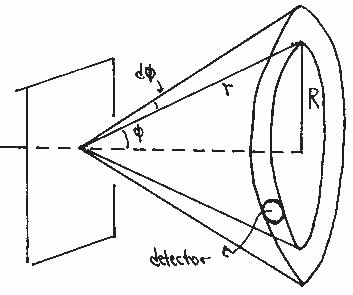
\includegraphics[width=2.375in,height=1.95833in]{images/04_rutherford/image020.jpg}
  \end{center}
  
  Therefore, by substituting for $dm$ the equation found above,
  \begin{equation*}
  y = \frac{Q \cdot dm}{2\pi r^2\sin(\phi)\,d\phi} = \frac{Q\pi ntb^2\cot(\phi/2)\csc^2(\phi/2)\,d\phi}{8\pi r^2\sin(\phi)\,d\phi}
  \end{equation*}
  Apply the trigonometric identity $\sin 2a = 2 \sin a \cos a$, where
  $\phi/2 = a$ (\emph{n.b.}: the identity is a simpler form of the identity,
  $\sin (a+b) = \sin a \cos b + \cos a \sin b$), and it follows that,
  \begin{equation*}
  y = \frac{Qntb^2\cot(\phi/2)\csc^2(\phi/2)}{16r^2\sin(\phi/2)\cos(\phi/2)} = \frac{Qntb^2\cos(\phi/2)\csc^2(\phi/2)}{16r^2\sin^2(\phi/2)\cos(\phi/2)}
  \end{equation*}
  which reduces to Rutherford's formula (5).]}
\end{equation}


Since
\begin{equation*}
b = 2NeE / mu^2 , \footnote{{[}Derived in note 13
  above.{]}}
\end{equation*}
we see from this equation that a number of $\alpha$~particles
(scintillations) per unit area of zinc sulphide screen at a given
distance $r$ from the point of incidence of the rays is
proportional to

\begin{quote}
(1) cosec\textsuperscript{4}($\phi$/2) or
1/$\phi$\textsuperscript{4} if $\phi$ be small;

(2) thickness of scattering material $t$ provided this is small

(3) magnitude of central charge $Ne$ {[}squared{]}

(4) and is inversely proportional to $(mu^2)^2$, or to the fourth
power of the velocity if $m$ be constant.
\end{quote}

In these calculations, it is assumed that the $\alpha$ particles
scattered through a large angle suffer only one large deflexion. For
this to hold, it is essential that the thickness of the scattering
material should be so small that the chance of a second encounter
involving another large deflection is very small. If, for example, the
probability of a single deflexion $\phi$ in passing through a
thickness $t$ is 1/1000, the probability of two successive
deflexions each of value $\phi$ is $1/10^6$, and is negligibly small.

The angular distribution of the $\alpha$~particles scattered from a thin
metal sheet affords one of the simplest methods of testing the general
correctness of this theory of single scattering. This has been done
recently for $\alpha$ rays by Dr. Geiger, who found that the
distribution for particles deflected between 30$^\circ$ and 150$^\circ$ from a thin
gold-foil was in substantial agreement with the theory. A more detailed
account of these and other experiments to test the validity of the
theory will be published later.\\
\centerline{* * *}
%
\subsection*{Comparison of Theory with Experiments}

Geiger{[}'s experiments{]} showed that the most probable angle of
deflection for an atom was nearly proportional to its atomic weight. It
consequently follows that the value of $N$ for different atoms
should be nearly proportional to their atomic weights, at any rate for
atomic weights between gold and aluminum.

Since the atomic weight of platinum is nearly equal to that of gold, it
follows from these considerations that the magnitude of the diffuse
deflexion of $\alpha$ particles through more than $90^\circ$ from gold and the
magnitude of the average small angle scattering of a pencil of rays in
passing through gold-foil are both explained on the hypothesis of single
scattering by supposing the atom of gold has a central charge of about
$100e$.\\
\centerline{* * *}
%
\subsection*{General Considerations}

In comparing the theory outlined in this paper with the experimental
results, it has been supposed that the atom consists of a central charge
supposed concentrated at a point, and that the large single deflexions
of the $\alpha$~and $\beta$~particles are mainly due to their passage
through the strong central field. The effect of the equal and opposite
compensating charge supposed distributed uniformly throughout a sphere
has been neglected. Some evidence in support of these assumptions will
now be briefly considered. For concreteness, consider the passage of a
high speed $\alpha$ particle through an atom having a positive central
charge $Ne$, and surrounded by a compensating charge of $N$
electrons. Remembering that the mass, momentum, and kinetic energy of
the $\alpha$~particle are very large compared to the corresponding
values for an electron in rapid motion, it does not seem possible from
dynamic considerations that an $\alpha$ particle can be deflected
through a large angle by a close approach to an electron, even if the
latter be in rapid motion and constrained by strong electrical forces.
It seems reasonable to suppose that the chance of single deflexions
through a large angle due to this cause, if not zero, must be
exceedingly small compared with that due to the central charge.

It is of interest to examine how far the experimental evidence throws
light on the question of the extent of the distribution of the central
charge. Suppose, for example, the central charge to be composed of
$N$ unit charges distributed over such a volume that the large
single deflexions are mainly due to the constituent charges and not to
the external field produced by the distribution. It has been shown that
the fraction of the $\alpha$ particles scattered through a large angle
is proportional to $(NeE)^2$, where $Ne$ is the central charge
concentrated at a point and $E$ the charge on the deflected
particle. If, however, this charge is distributed in single units, the
fraction of the $\alpha$ particles scattered through a given angle is
proportional to $Ne^2$ instead of $N^2e^2$.\footnote{{[}Proportionality
  to $Ne^2$ had been derived by Thomson for his atom-model.{]}} In
this calculation, the influence of mass of the constituent particle has
been neglected, and account has only been taken of its electric field.
Since it has been shown that the value of the central point charge for
gold must be about 100, the value of the distributed charge required to
produce the same proportion of single deflexions through a large angle
should be at least 10,000. Under these conditions the mass of the
constituent particle would be small compared with that of the
$\alpha$~particle, and the difficulty arises of the production of large
single deflections at all. In addition, with such a large distributed
charge, the effect of compound scattering is relatively more important
than that of single scattering. For example, the probable small angle of
deflexion of a pencil of $\alpha$~particles passing through a thin
gold-foil would be much greater than that experimentally observed by
Geiger. The large and small angle scattering could not then be explained
by the assumption of a central charge of the same value. Considering the
evidence as a whole, it seems simplest to suppose that the atom contains
a central charge distributed through a very small volume, and that the
large single deflexions are due to the central charge as a whole, and
not to its constituents. At the same time, the experimental evidence is
not precise enough to negative the possibility that a small fraction of
the positive charge may be carried by satellites extending some distance
from the centre. Evidence on this point could be obtained by examining
whether the same central charge is required to explain the large single
deflexions of $\alpha$ and $\beta$~particles; for the $\alpha$~particle
must approach much closer to the centre of the atom than the $\beta$
particle of average speed to suffer the same large deflexion.

The general data available indicate that the value of this central
charge for different atoms is approximately proportional to their atomic
weights, at any rate for atoms heavier than aluminum. It will be of
great interest to examine experimentally whether such a simple relation
holds also for the lighter atoms. In cases where the mass of the
deflecting atom (for example, hydrogen, helium, lithium) is not very
different from that of the $\alpha$ particle, the general theory of
single scattering will require modification, for it is necessary to take
into account the movements of the atom itself\footnote{{[}Compare
  Newton, \emph{Principia}, Book I, Props. 57-60, in which corrections
  are made for the motion of the central body.{]}}...

The deductions from the theory so far considered are independent of the
sign of the central charge, and it has not so far been found possible to
obtain definite evidence to determine whether it be positive or
negative. It may be possible to settle the question of sign by
consideration of the difference of the laws of absorption of the
$\beta$ particle to be expected on the two hypotheses, for the effect
of radiation in reducing the velocity of the $\beta$ particle should be
far more marked with a positive than with a negative centre. If the
central charge be positive, it is easily seen that a positively charged
mass, if released from the centre of a heavy atom, would acquire a great
velocity in moving through the electric field. It may be possible to
account in this way for the high velocity of $\alpha$~particles without
supposing that they are initially in rapid motion within the
atom.\footnote{{[}The conjecture of a positive central charge was
  confirmed in later work, lending credence to the hypothesis that the
  alpha particles ejected by radium and other radioactive materials
  originate in the atomic \emph{nuclei} of those materials. The
  $\alpha$-particle itself could now be understood to be the
  \emph{``bare'' nucleus, without the surrounding electrons}, of a
  helium atom. This accounted both for its +2 charge and for its
  extremely small size.{]}}

Further consideration of the application of this theory to these and
other questions will be reserved for a later paper, when the main
deductions of the theory have been tested experimentally. Experiments in
this direction are already in progress by Geiger and Marsden.

\section*{Geiger and Marsden's Experiments}

The most decisive experimental work corroborating the theory Rutherford 
developed was reported by Geiger and Marsden in 1913. We
quote from the introduction to their report in \emph{Philosophical
Magazine} \textbf{25} (1913), 604--623; reprinted in \emph{The World of The
Atom}, vol.\ I, 722--733:

\begin{quote}
At the suggestion of Prof. Rutherford, we have carried out experiments
to test the main conclusions of the above theory. The following points
were investigated:---


(1) Variation with angle.

(2) Variation with thickness of scattering material.

(3) Variation with atomic weight of scattering material.

(4) Variation with velocity of incident $\alpha$ particles.

(5) The fraction of particles scattered through a definite angle.

The main difficulty of the experiments has arisen from the necessity of
using a very intense and narrow source of $\alpha$ particles owing to
the smallness of the scattering effect. All the measurements have been
carried out by observing the scintillations due to the scattered
$\alpha$~particles on a zinc-sulphide screen, and during the course of
the experiments over 100,000 scintillations have been counted. It may be
mentioned in anticipation that all the results of our investigation are
in good agreement with the theoretical deductions of Prof. Rutherford,
and afford strong evidence of the correctness of the underlying
assumption that an atom contains a strong charge at the centre, of
dimensions small compared with the diameter of the atom.
\end{quote}

\section*{Experiment: Rutherford Scattering of $\alpha$ particles}

The College has built a scattering apparatus which can provide a rough
test of the hypothesis of the concentration of positive charge in the atom. 
Our apparatus includes an alpha
particle source that is directed toward a piece of gold foil; on the far
side of the foil is placed a detector. Our object is to measure how
frequently alpha particles are deflected at high angles, from 30 to 70
degrees. In our apparatus, however, rather than moving the detector, the
alpha particle source and the foil sit on an arm that swivels, and we
jointly move the particle source and foil in order to adjust the angle
between the far surface of the foil and the detector (which remains
fixed). The College's apparatus is not as precise as Geiger and
Marsden's, primarily because our alpha particle source is weak compared
to theirs.\footnote{Theirs was ``hot enough to cook a chicken,''
  according to a knowledgeable commentator.} In addition, the beam of
alpha particles is relatively wide, about thirty degrees (in
measurements taken without the gold foil in place, the detector records
about 200 counts per second at the center of the beam, and 100 counts
per second up to six or seven degrees to each side of the center).
Nevertheless, the apparatus is sufficiently precise to test Rutherford's
statement that, at a given angle $\phi$, the number of alpha particles
detected per unit area and per unit time will be proportional to
cosec\textsuperscript{4}($\phi$ /2).

Although long angle deflections are more probable than Thomson's model
of the atom would suggest, they are still relatively rare, so that
measurements need to be taken over a long period of time. In the late
afternoon lab assistants will set the angle of the detector and reset
the counter to zero, and then read the counter the following morning.
Readings will be taken between 30 and 70 degrees at intervals of 10
degrees.

During class, one may take readings at short angles, between 0 and 30
degrees, for short periods of time (between 20 and 200 seconds, using
longer periods for longer angles). These readings cannot be used to
confirm Rutherford's mathematical prediction of the probability of
deflections, but they can be compared to readings previously taken
\emph{without the gold foil in place} in order to observe, in general
terms, the effect of the foil on the alpha particle beam.

%\includegraphics[width=5.5283in,height=3.24858in]{media/image22.png}
